\documentclass[a4paper, reqno]{amsart}
\usepackage{amssymb,amscd,amsfonts,amsbsy,nicefrac,mathtools}
\usepackage[utf8]{inputenc}
\usepackage{amsmath,amsthm,amssymb,amsfonts,enumitem}
\usepackage[pdftex]{graphicx,color}
\usepackage{tikz}
\usepackage[T1]{fontenc}

\begin{document}

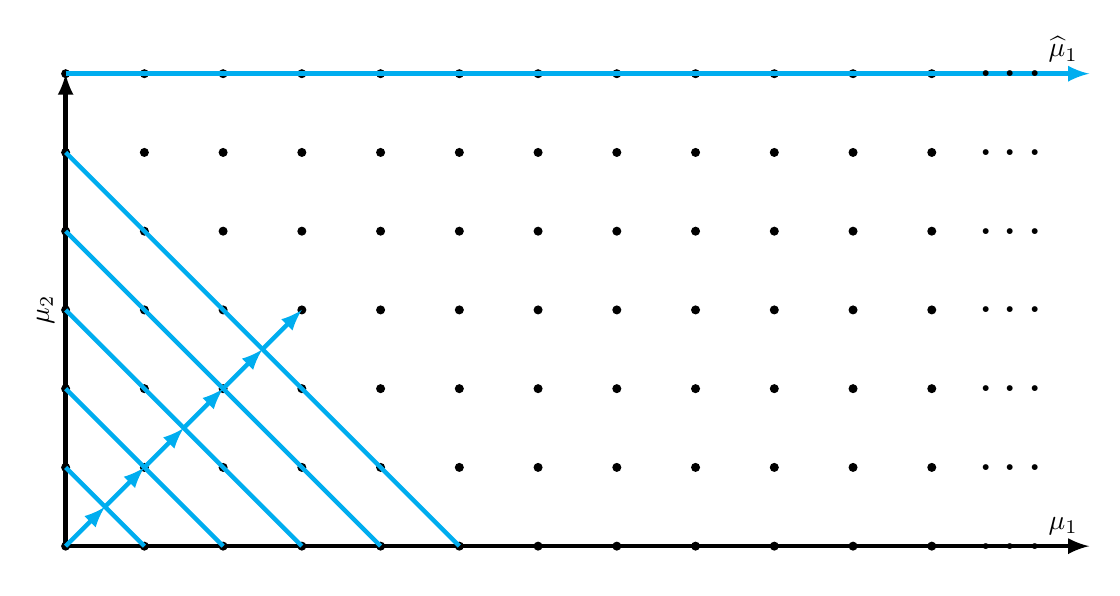
\begin{tikzpicture}

\foreach \x in {0,1,...,11}{
\foreach \y in {0,1,...,6}{
\node[draw,circle,inner sep=1pt,fill] at (\x,\y) {};}}
\draw [ultra thick,-latex,black] (0,0) -- (0,6) node[midway,above,sloped] {$\mu_2$};
\draw [ultra thick,-latex,black] (0,0) -- (13,0) node [above left] {$\mu_1$};
\draw [ultra thick,-latex,cyan] (0,6) -- (13,6) node [above left,black] {$\widehat{\mu}_1$};
\draw [ultra thick,cyan] (1,0) -- (0,1);
\draw [ultra thick,cyan] (2,0) -- (0,2);
\draw [ultra thick,cyan] (3,0) -- (0,3);
\draw [ultra thick,cyan] (4,0) -- (0,4);
\draw [ultra thick,cyan] (5,0) -- (0,5);
\draw [ultra thick,-latex,cyan] (0,0) -- (0.5,0.5) node{} [above left];
\draw [ultra thick,-latex,cyan] (0.5,0.5) -- (1,1) node{} [above left];
\draw [ultra thick,-latex,cyan] (1,1) -- (1.5,1.5) node{} [above left];
\draw [ultra thick,-latex,cyan] (1.5,1.5) -- (2,2) node{} [above left];
\draw [ultra thick,-latex,cyan] (2,2) -- (2.5,2.5) node{} [above left];
\draw [ultra thick,-latex,cyan] (2.5,2.5) -- (3,3) node{} [above left];
\node[scale=2] at (12,0) {$\ldots$};
\node[scale=2] at (12,1) {$\ldots$};
\node[scale=2] at (12,2) {$\ldots$};
\node[scale=2] at (12,3) {$\ldots$};
\node[scale=2] at (12,4) {$\ldots$};
\node[scale=2] at (12,5) {$\ldots$};
\node[scale=2] at (12,6) {$\ldots$};

\end{tikzpicture}

\end{document}